documentclass[../main.tex]{subfiles}
 
\begin{document}
\textbf{Indels in \textit{Armillaria gallica}}

In order to start exploring InDels, a mpileup file was made for all 15 strains. This was done by using the command in samtools \textit{mpileup}. A pileup file is a text-based format for summarizing the calls of aligned reads to the reference sequence. This format also allows for visual displays of SNP/indel calling and alignments. Once, a pileup file was produced. It is at this point, where output tags were included into the data. These output tags will indicate the read depth, quality score and also anything else that may be of use for analysis.  A package called \textit{BCFtools} was implemented. BCFtools is a set of utilities that manipulate variant calls in the variant call format (vcf) as well as its binary counterpart (bcf). The pileup file was indexed using the command \textit{bcftools index}. This creates an index of the sequence from the pileup file. After this is done, we use the command \textit{bcftools call}, which is the variant calling. This will call the indels in this case and produce a .vcf and a .bcf file which show the indels and their locations. The script which does this process is called \textit{ctq_reads_find_indels.sh}. 

It appears at first glance that there was many indels detected that were the same throughout the strains as seen in \ref{tab:sum_indel}. The summary table only shows the first three indels found within the each strain, however throughout the data, this is a repeated pattern. 

\begin{table}[H]
	\begin{center}
		\vspace{-1.5cm}
		\begin{singlespace}
			\captionof{table}[Summary Indel Table]{A summary table of the first three indels found in each of the strains which includes the scaffold number, the location at which the indel is found, the number of reads that support that indel, and the raw read depth\\} \label{tab:sum_indel}
			\scalebox{.9}{
				\begin{tabular}{ |c|c|c|c|c|c|c| } 
					\hline
					Strain No. & Scaffold No. & Location & No. of Reads Supporting & Raw Read Depth \\
					\hline
					\multirow{3}{4em}{Ar73} & 1 & 7762 &54 & 156\\
					&1 & 10784 & 34 & 148\\
					&1 & 12340 & 37 & 123\\
					\hline
					\multirow{3}{4em}{Ar109} & 1 & 7762 & 56 & 163\\
					& 1 & 10784 & 68 & 175 \\
					& 1 & 16154 & 7 & 176 \\
					\hline
					\multirow{3}{4em}{Ar119} & 1 & 7762 & 62 & 163 \\
					& 1 & 10784 & 57 & 140 \\
					& 1 & 16154 & 4 & 167 \\
					\hline
					\multirow{3}{4em}{Ar142} & 1 & 7762 & 63 & 189 \\
					& 1 & 10784 & 55 & 186 \\
					& 1 & 16154 & 5 & 125 \\
					\hline
					\multirow{3}{4em}{Ar159} & 1 & 7762 & 41 & 116 \\ 
					& 1 & 10784 & 28 & 100  \\ 
					& 1 & 16154 & 3 & 85 \\ 
					\hline
					\multirow{3}{4em}{Ar170} & 1 & 7762 & 73 & 222 \\ 
					& 1 & 10784 & 61 & 194  \\ 
					& 1 & 12340 & 72 & 193 \\ 
					\hline
					\multirow{3}{4em}{Ar174} & 1 & 7762 & 63 & 201 \\ 
					& 1 & 9593 & 72 & 218  \\ 
					& 1 & 10784 & 45 & 184 \\ 
					\hline
					\multirow{3}{4em}{Ar175} & 1 & 7762 & 47 & 141 \\ 
					& 1 & 10784 & 28 & 108  \\ 
					& 1 & 12340 & 35 & 102 \\ 
					\hline
					\multirow{3}{4em}{Ar176} & 1 & 7762 & 39 & 141 \\ 
					& 1 & 9593 & 43 & 129  \\ 
					& 1 & 10784 & 33 & 115 \\ 
					\hline
					\multirow{3}{4em}{Ar179} & 1 & 7762 & 63 & 193 \\ 
					& 1 & 9593 & 64 & 205  \\ 
					& 1 & 10784 & 50 & 195 \\ 
					\hline
					\multirow{3}{4em}{Ar188} & 1 & 7762 & 17 & 62 \\ 
					& 1 & 10784 & 11 & 47  \\ 
					& 1 & 12340 & 24 & 54 \\ 
					\hline
					\multirow{3}{4em}{Ar194} & 1 & 7762 & 35 & 133 \\ 
					& 1 & 10784 & 32 & 105  \\ 
					& 1 & 12340 & 35 & 110 \\ 
					\hline
					\multirow{3}{4em}{Ar196} & 1 & 7762 & 72 & 224 \\ 
					& 1 & 10784 & 53 & 169  \\ 
					& 1 & 12340 & 72 & 192 \\ 
					\hline
					\multirow{3}{4em}{Ar201} & 1 & 7762 & 38 & 110 \\ 
					& 1 & 10784 & 44 & 116  \\ 
					& 1 & 12340 & 50 & 102 \\ 
					\hline
					\multirow{3}{4em}{Ar213} & 1 & 7762 & 76 & 220 \\ 
					& 1 & 9593 & 63 & 196  \\ 
					& 1 & 10784 & 48 & 188 \\ 
					\hline
				\end{tabular}
			}
		\end{singlespace}
	\end{center}
\end{table}

\subsection{Read Depth of Indels}

Read depth or sequence depth was one of the output tags that we added to the pileup file previously. Read depth was important in this analysis thus, we decided to explore the them as part of the indel analysis. Since, it was already one of the output tags we previously added, it was a very simple as to extract the datapoint with the corresponding scaffold and location. These were plotted as to see which regions or scaffolds had the highest read depth and to see if the read depth overall was appropriate for further directions.

It was shown that there was good read depth generally throughout the scaffolds. The larger the scaffold, the more indels occured however, the read depth still holds to be good. 

\begin{figure}[H]
	\begin{centering}
		\vspace{1.5cm}
		\resizebox{78mm}{78mm}{\includegraphics[angle=0,width=1.0\linewidth]{Figures/1_DP_locat
				ions.pdf}}
		\resizebox{78mm}{78mm}{\includegraphics[angle=0,width=1.0\linewidth]{Figures/50_DP_loca
				tions.pdf}}\\
		\resizebox{78mm}{78mm}{\includegraphics[angle=0,width=1.0\linewidth]{Figures/100_DP_loc
				ations.pdf}}
		\resizebox{78mm}{78mm}{\includegraphics[angle=0,width=1.0\linewidth]{Figures/211_DP_loc
				ations.pdf}}
		\begin{singlespace}
			\vspace{-0.5cm}
			\caption[The Read Depth of Indels Found]{The Read Depth of Indels Found in Ar109 at scaffold 1, 50, 100 and 211
				t Scaffold:1, 50, 100, and 211. Every datapoint indicates one indel}\label{readdepth_indel}
		\end{singlespace}
	\end{centering}
\end{figure}

\subsection{Indel Lengths}  

Since given the read depths, it was shown that it would be appropriate to move forward. The next step we did was analyze the difference lengths of the indels. This was done by using a very simple command from the package vcftools, the command was \textit{--hist-indel-len}. This gave a very crude histogram as well as the counts for each indel at each length. From this data we created a better visualization of the data. 

It can be seen that the smaller the indel, the more frequent it occurs. This holds true throughout the strains that were tested.

\begin{figure}[H]
	\begin{centering}
		\vspace{-1.5cm}
		\resizebox{78mm}{78mm}{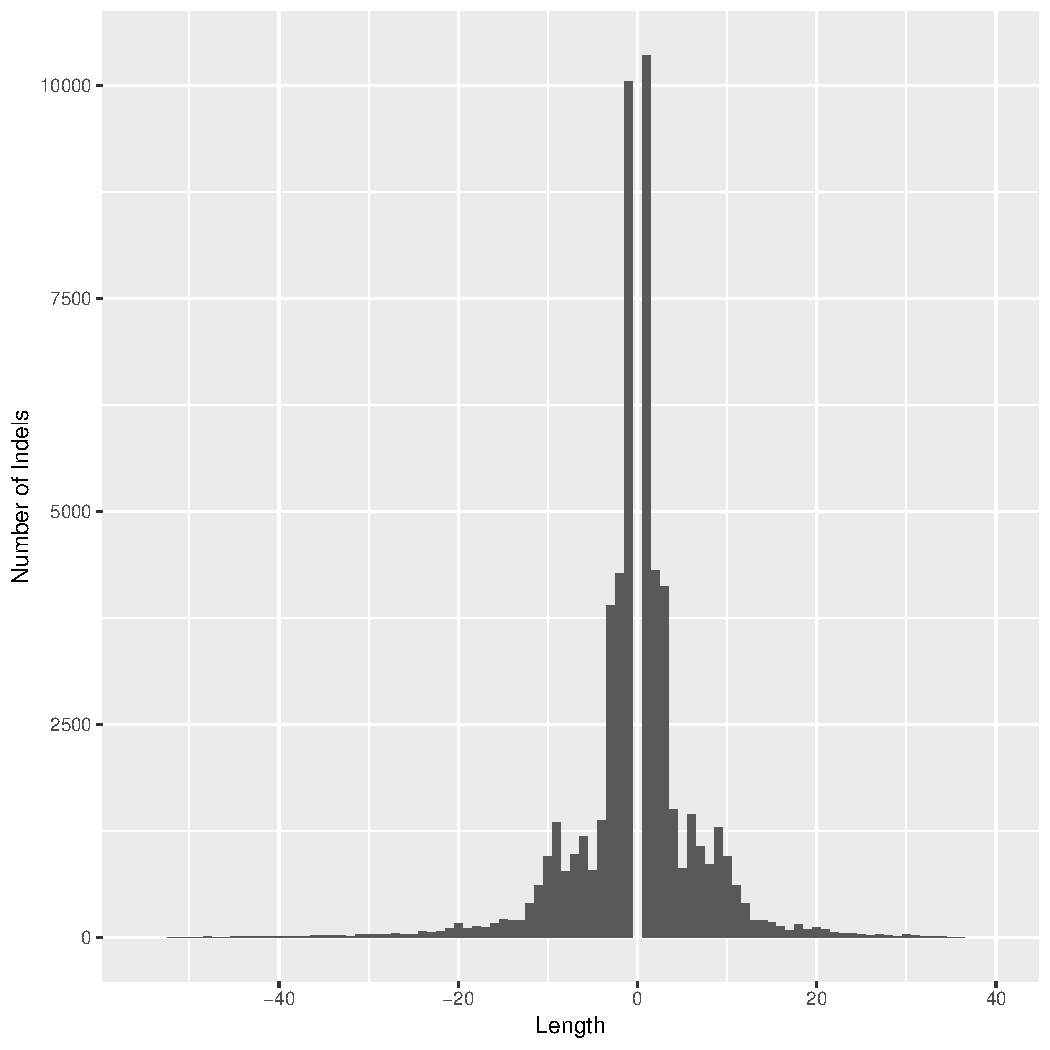
\includegraphics[angle=0,width=0.75\linewidth]{Figures/Ar109_histogram.pdf}}
		\resizebox{78mm}{78mm}{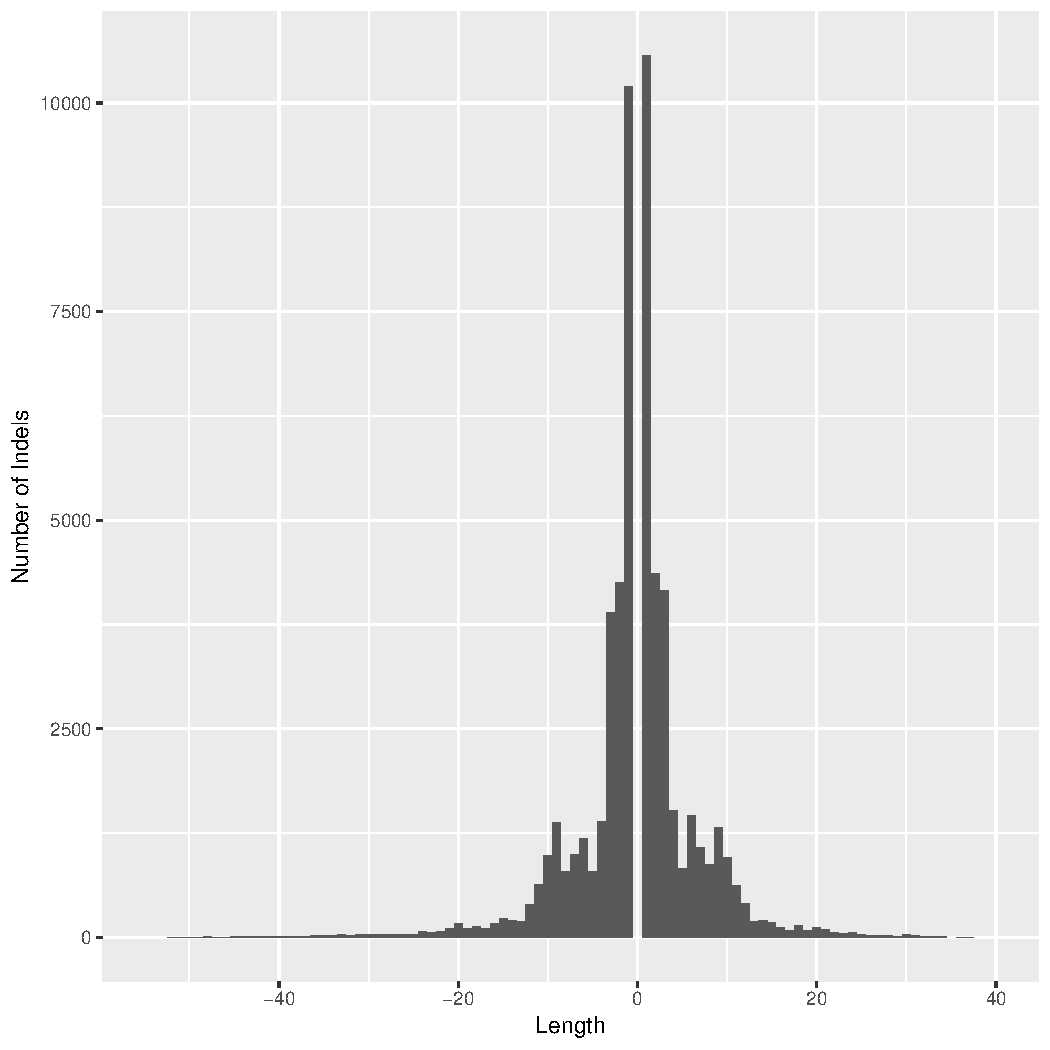
\includegraphics[angle=0,width=0.75\linewidth]{Figures/Ar119_histogram.pdf}}\\
		\begin{singlespace}
			\vspace{-0.5cm}
			\caption[The Frequency of the Indel Length]{The Frequency of the Indel Length Per Strain, Ar109 and Ar119}\label{Length_Indel_His}
		\end{singlespace}
	\end{centering}
\end{figure}
 
 
In the histograms, it can be seen that the largest indels were found to be single nucleotide bases. It was a bell-shaped or a normal distrubution, which is what to be expected. From this, we focused on the extremities of the indels. We explored on the largest insertions detected. We extracted the sequences and the 5 nucleotides that flanked each end, and BLAST-ed these against the NCBI database.  

Many of the BLAST searchs came back as empty however, there were a couple of hits throughout the data. We also found many repeated elements within the indel analysis. One BLAST hit that was further looked into was at position 117162 at scaffold 98. It was 44 nucleotides long, which still is not that large in the grand scheme of indels. However, it was a perfect match against \textit{Streptomyces actuosus}. This indel was found in 8 of the 15 strains that were tested. Using the literature, we indicated where this indel was found on the spatial map as well as the phylogeny.
 
 
\begin{figure}[H]
	\begin{centering}
		\vspace{1.5cm}
		\resizebox{78mm}{78mm}{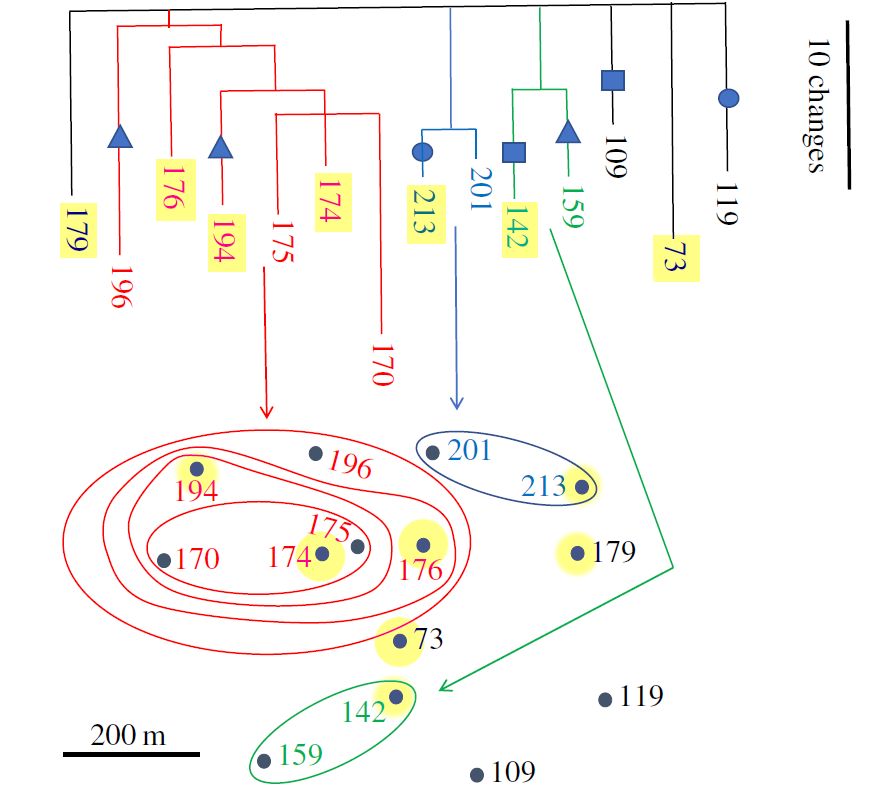
\includegraphics[angle=0,width=1.0\linewidth]{Figures/tree_dd.png}}
		\begin{singlespace}
			\vspace{-0.5cm}
			\caption[Phylogeny overlap with \textit{Streptomyces} Indels]{The phylogeny found within the original publication (Anderson \textit{et al}, 2018) with the indication of where the \textit{Steptomyces} Indel was found}\label{tree1}
		\end{singlespace}
	\end{centering}
\end{figure}

\begin{figure}[H]
	\begin{centering}
		\vspace{1.5cm}
		\resizebox{78mm}{78mm}{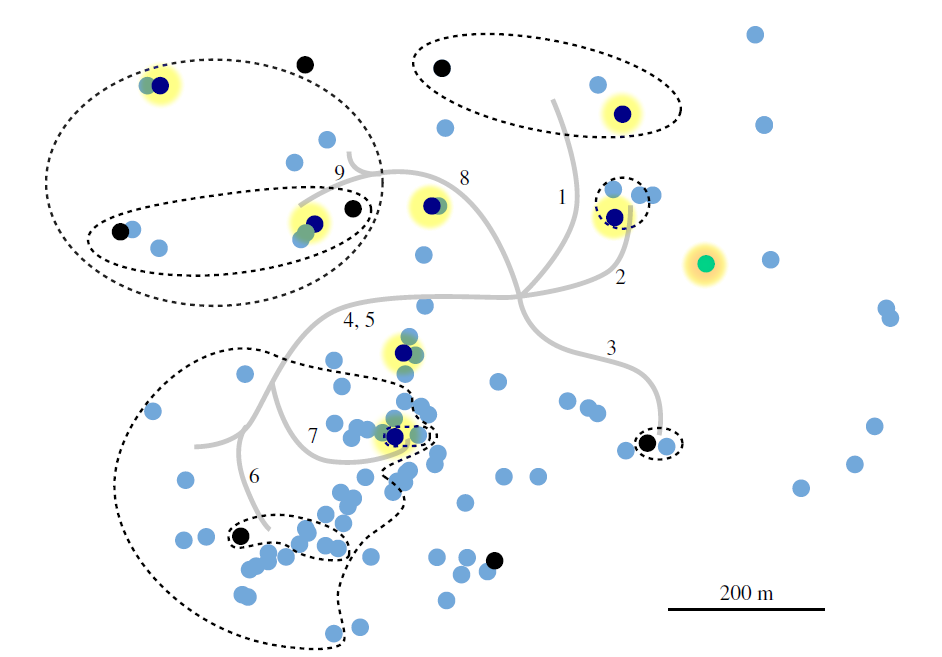
\includegraphics[angle=0,width=1.0\linewidth]{Figures/tree_dd2.png}}
		\begin{singlespace}
			\vspace{-0.5cm}
			\caption[Spatial map overlap with \textit{Streptomyces} Indels]{The spatial map found within the original publication (Anderson \textit{et al}, 2018) with the indication of where the \textit{Steptomyces} Indel was found}\label{tree2}
		\end{singlespace}
	\end{centering}
\end{figure}

In order to show a better representation, we included the actual sequence of the found indel and the flanking regions around it. In the sequences where the indel is not present, the sequence would be linear.


\begin{figure}[H]
	\begin{centering}
		\vspace{1.5cm}
		\resizebox{78mm}{78mm}{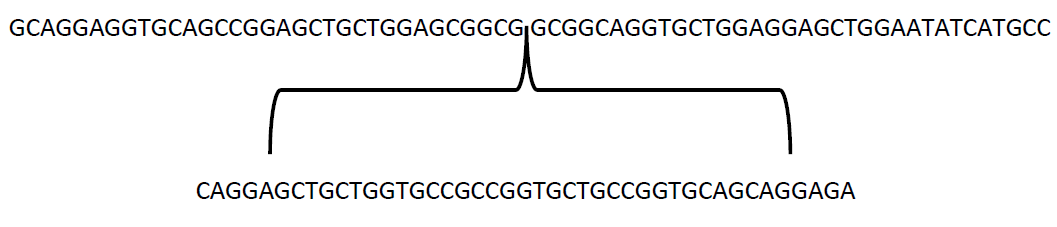
\includegraphics[angle=0,width=1.0\linewidth]{Figures/177162.png}}
		\begin{singlespace}
			\vspace{-0.5cm}
			\caption[Sequence with \textit{Streptomyces} Indel]{The placement of the found indel in the sequence of the reference genome}\label{seqindel}
		\end{singlespace}
	\end{centering}
\end{figure}


\end{document}